\documentclass[Main]{subfiles}
\begin{document}

\section{Deployment View}
Systemet består af en fjernbetjening, dronen, samt modtagerenheden på dronen, vist på Figur \ref{Fig:DeploymentViewOverview}.
\fxnote{Er det her knap beskrivelsen skal være?}

\begin{figure}[H]
\centering
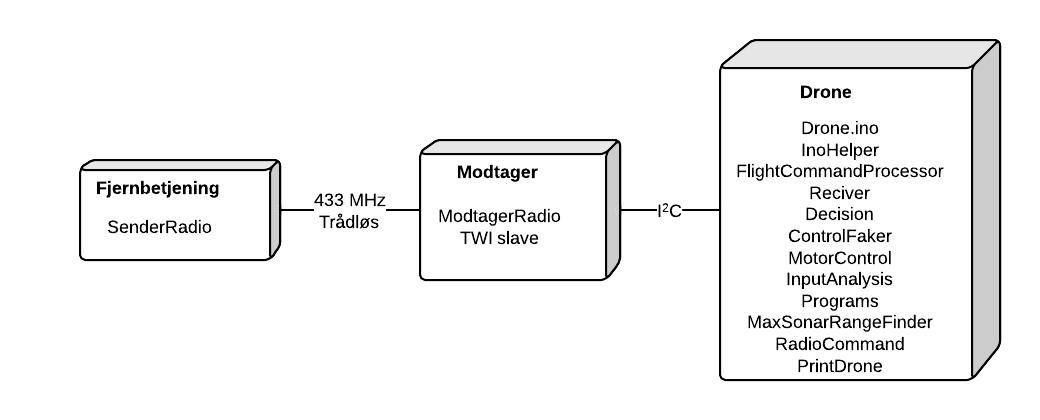
\includegraphics[width = 0.90 \textwidth]{DeploymentViewOverview}
\caption{Deployment View diagram}
\label{Fig:DeploymentViewOverview}
\end{figure}

Fjernbetjeningen sender en frame til dronen vha. det trådløse 433 MHz signal, som opfanges af modtager-enheden.
Herefter bliver pakken lagt over i en output buffer til dronen som. Dronen kan så hente denne pakke når den har tid til det. 
Kommunikationen mellem dronen og modtageren er gennem \itoc-protokollen.


\newpage
\subsection{Protokoller}
En kort beskrivelse af protokollerne mellem de forskellige enheder.

\subsubsection{Fjernbetjening til modtager}
Ved tryk på knapperne på fjernbetjeningen sendes et frame til modtageren.
Signalet består af 2 bytes, hvoraf det første er en programindikator og den anden er selve programmet.

Kommandoer der kan sendes vises i Tabel \ref{Tab:kommando}.

\begin{table}[H]
  \centering
	\begin{tabular}{l l}
	\hline
	\textbf{Kommando} 	& \textbf{Indhold i bytes} \\ \hline
	Let 				& \code{0x03} + \code{0x3F} + \code{0x02} \\
	Autoland 			& \code{0x03} + \code{0x3F} + \code{0x04} \\
	Fremad 				& \code{0x03} + \code{0x3F} + \code{0x08} \\
	Roter til højre 	& \code{0x03} + \code{0x3F} + \code{0x0A} \\
	Roter til venstre 	& \code{0x03} + \code{0x3F} + \code{0x0C} \\
	Roter til højre 	& \code{0x03} + \code{0x3F} + \code{0x0E} \\
	Stop 				& \code{0x03} + \code{0x3F} + \code{0x10} \\
	Inkrementer højde 	& \code{0x03} + \code{0x3F} + \code{0x12} \\
	Dekrementer højde 	& \code{0x03} + \code{0x3F} + \code{0x14} \\ \hline	
  	\end{tabular}  
\caption{Kommandoer sendt sender og modtager.}
\label{Tab:kommando}
\end{table}




\newpage
\subsubsection{Modtager til drone}
Når et frame er modtaget på modtagerradioen, tjekker den framet for om CRC passer. 
Hvis der er uoverensstemmelse mellem størrelsen på frame og CRC værdien, bliver framet kasseret. 
Hvis framets størrelse og CRC stemmer overens, generer modtagerradioen et interrupt på µ-controller 2. 
µ-Controlleren vil så hente den modtagne pakke fra radioen og strippe den for pakke længde. 
Herefter vil den blive lagt ud i en output buffer til \itoc-forbindelsen til dronen, som nu kan hente den næste gang den har tid. 

Kommandoer der kan sendes vises i Tabel \ref{Tab:kommandoer}.

\begin{table}[H]
  \centering
	\begin{tabular}{l l}
	\hline
	\textbf{Kommando} 	& \textbf{Indhold i bytes} \\ \hline
	Let 				& \code{0x3F} + \code{0x02} \\
	Autoland 			& \code{0x3F} + \code{0x04} \\
	Fremad 				& \code{0x3F} + \code{0x08} \\
	Roter til højre 	& \code{0x3F} + \code{0x0A} \\
	Roter til venstre 	& \code{0x3F} + \code{0x0C} \\
	Roter til højre 	& \code{0x3F} + \code{0x0E} \\
	Stop 				& \code{0x3F} + \code{0x10} \\
	Inkrementer højde 	& \code{0x3F} + \code{0x12} \\
	Dekrementer højde 	& \code{0x3F} + \code{0x14} \\ \hline	
  	\end{tabular}  
\caption{Kommandoer sendt mellem modtager og drone.}
\label{Tab:kommandoer}
\end{table}


\end{document}